\documentclass{sig-alternate}

\usepackage{enumitem}
\usepackage{framed}
\usepackage{listings}
\usepackage{amstext}
\usepackage{amstext}
\usepackage{pdfpages}
\usepackage{alltt}
\usepackage{epstopdf}
\usepackage{xspace,colortbl}
\usepackage[USenglish]{babel}
\usepackage{multirow}
\usepackage{url}
\usepackage{subfigure}
\usepackage{graphicx}
\usepackage{amssymb}
\usepackage{fmtcount}
\usepackage{amsfonts}
\usepackage{xspace}
\usepackage{amsmath}
\usepackage{multirow}
\usepackage[mathscr]{eucal}
%\usepackage{psfrag}
\usepackage{colortbl}
\usepackage{bm}
\usepackage[nospace]{cite}


\usepackage[algoruled,vlined,linesnumbered]{algorithm2e}
\usepackage{xcolor}
\newcommand\mycommfont[1]{\scriptsize\ttfamily\textcolor{blue}{#1}}
\SetCommentSty{mycommfont}
\SetKwFor{ParForAll}{for}{do in parallel}{end}
\SetKw{WaitUntil}{wait until}


\lstset{basicstyle=\scriptsize,breaklines=true}

\linespread{0.94}%

\makeatletter
\def\@copyrightspace{\relax}
\makeatother

\begin{document}

\setlength{\belowdisplayskip}{2pt} \setlength{\belowdisplayshortskip}{2pt}
\setlength{\abovedisplayskip}{2pt} \setlength{\abovedisplayshortskip}{2pt}
\setlength{\belowcaptionskip}{-8pt}
\selectfont

\newtheorem{theorem}{Theorem}
\newtheorem{example}{Example}
\newtheorem{definition}{Definition}
\newtheorem{proposition}{Proposition}
\newtheorem{lemma}{Lemma}
\newtheorem{corollary}{Corollary}

\newcommand{\cond}{\textrm{Cond}\xspace}
\newcommand{\dataset}{data set\xspace}
\newcommand{\datasets}{data sets\xspace}
\newcommand{\spview}{\textsf{SPView}\xspace}
\newcommand{\fjview}{\textsf{FJView}\xspace}
\newcommand{\aggview}{\textsf{AggView}\xspace}
\newcommand{\hashfunc}[1]{\textsf{hashfunc}(#1)\xspace}

\newcommand{\avgfunc}{\ensuremath{\texttt{avg} }\xspace}
\newcommand{\maxfunc}{\ensuremath{\texttt{max} }\xspace}
\newcommand{\minfunc}{\ensuremath{\texttt{min} }\xspace}
\newcommand{\histfunc}{\ensuremath{\texttt{histogram\_numeric} }\xspace}
\newcommand{\countfunc}{\ensuremath{\texttt{count}}\xspace}
\newcommand{\sumfunc}{\ensuremath{\texttt{sum} }\xspace}
\newcommand{\varfunc}{\ensuremath{\texttt{var} }\xspace}
\newcommand{\covfunc}{\ensuremath{\texttt{cov} }\xspace}
\newcommand{\corrfunc}{\ensuremath{\texttt{corr} }\xspace}
\newcommand{\medfunc}{\ensuremath{\texttt{median} }\xspace}
\newcommand{\percfunc}{\ensuremath{\texttt{percentile} }\xspace}
\newcommand{\havingfunc}{\ensuremath{\texttt{HAVING} }\xspace}
\newcommand{\ratio}{\ensuremath{\rho }\xspace}


\newcommand{\scp}{\textbf{SampleCleanPipeline}\xspace}
\newcommand{\sca}{\textbf{SampleCleanAlgorithm}\xspace}


\newcommand{\insertion}{\ensuremath{\texttt{INSERT} }\xspace}
\newcommand{\update}{\ensuremath{\texttt{UPDATE} }\xspace}
\newcommand{\delete}{\ensuremath{\texttt{DELETE} }\xspace}


\newcommand{\tbl}[1]{\textsf{#1}\xspace}
\newcommand{\field}[1]{\textsf{#1}\xspace}
\newcommand{\cost}{\textrm{cost}\xspace}
\newcommand{\ans}{\textsf{ans}\xspace}
\newcommand{\dans}{\Delta\textsf{ans}\xspace}
\newcommand{\cqp}{correction query processing\xspace}
\newcommand{\Cqp}{Correction query processing\xspace}

\newcommand{\reminder}[1]{{{\textcolor{magenta}{\{\{\bf #1\}\}}}\xspace}}
\newcommand{\specialcell}[2][c]{%
  \begin{tabular}[#1]{@{}c@{}}#2\end{tabular}}

\def\ojoin{\setbox0=\hbox{$\bowtie$}%
  \rule[-.02ex]{.25em}{.4pt}\llap{\rule[\ht0]{.25em}{.4pt}}}
\def\leftouterjoin{\mathbin{\ojoin\mkern-5.8mu\bowtie}}
\def\rightouterjoin{\mathbin{\bowtie\mkern-5.8mu\ojoin}}
\def\fullouterjoin{\mathbin{\ojoin\mkern-5.8mu\bowtie\mkern-5.8mu\ojoin}}

%\newcommand{\reminder}[1] {}
\pagestyle{plain}

\title{A Monte-Carlo Approach For Robust Execution of Heuristic Entity Resolution Pipelines}

\maketitle


\vspace{-1em}

\begin{abstract}
\reminder{TODO}
\end{abstract}


% !TEX root = demo.tex
\section{Introduction}\label{sec:intro}

\begin{figure}[t]
\centering
\vspace{-0.5cm}
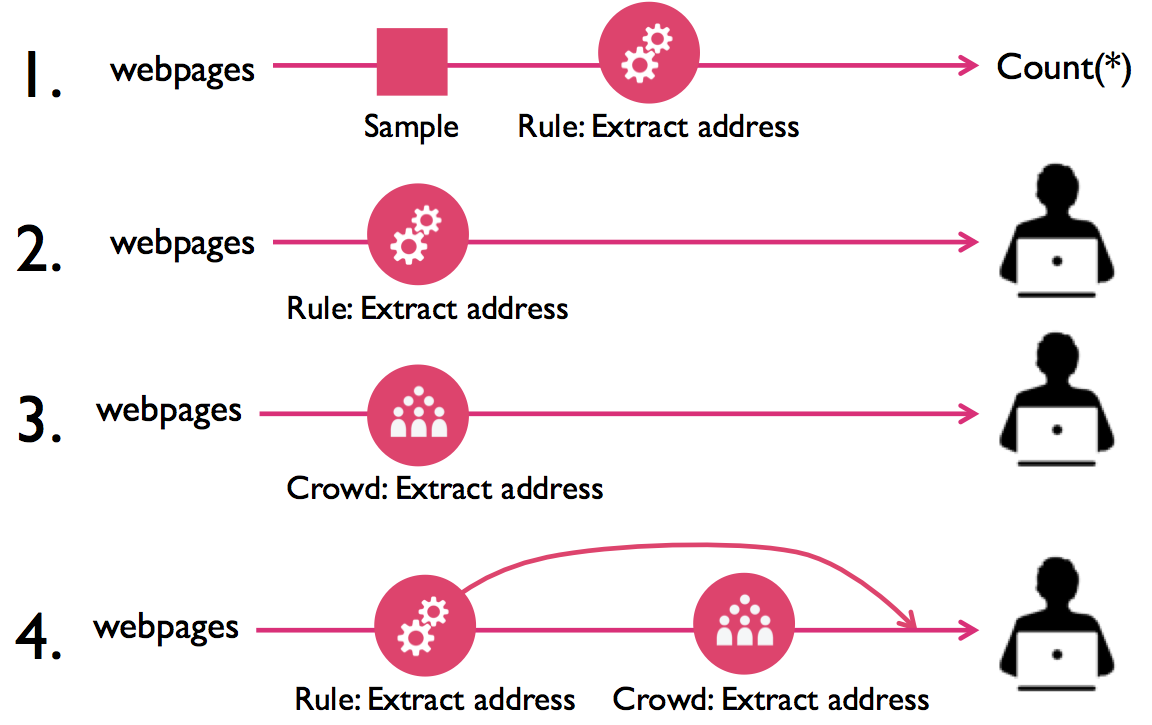
\includegraphics[width = .4\textwidth]{figs/lifecycle.png}
\vspace{-0.4cm}
\caption{Example iterations on the design of the portion of a cleaning plan that extracts restaurant addresses from their unstructured webpages.  
1) An exploratory plan that uses a sample to evaluate a simple address extraction method.
2) A plan that applies the method to the entire dataset. The quality is unsatisfactory. 
3) An alternate plan that uses manual crowd extraction. The quality is now high, but the crowd-based extractor is slow. 
4) A hybrid plan that sends only difficult webpages to the crowd, maximizing accuracy without sacrificing latency.}
\label{fig:ex-plan}
\vspace{-0.3cm}
\end{figure}
% why feedback loops exist/are important (cite Joe’s shit in the past 3 years, blinkdb, etc.). highlight domain specificity. Large variety of data cleaning tasks

%
% General comment that data cleaning is important:
%
The ease of acquiring and merging many large-scale data sources has led to a prevalence of dirty data.
Unfortunately, blindly using results that are derived from dirty data can lead to hidden yet significant errors in modern data-driven applications, so data must be cleaned before it is used.
But because data cleaning is often specific to the domain, dataset, and eventual analysis, analysts report spending upwards of 80\% of their time on problems in data cleaning~\cite{kandel2012}.
The analyst is faced with a breadth of possible errors that are manifest in the data and a variety of options to resolve them.
She must go through the cleaning process via trial and error, deciding for each of her data sources what to extract, how to clean it, and whether that cleaning will significantly change results.

Data cleaning is inherently iterative and Figure~\ref{fig:ex-plan} shows a common progression for the development of a data cleaning plan, in this case the extraction of a restaurant's address from its unstructured webpage.
While this operation can easily be represented at a \textit{logical} level by its input and output schema, there is a huge space of possible \textit{physical} implementations of the logical operators. 
For example, extraction could depend on manually specified rules (\textit{rule-based}), use models trained on previously extracted ground truth records (\textit{learning-based}), ask crowd workers to extract the desired data fields (\textit{crowd-based}), or some combination of the three (e.g., active learning, which uses crowd workers to provide labels for a learning-based approach).
Even after selecting (say) a crowd-based operator, many parameters might influence the quality of the output data or the speed and cost of cleaning: the number of crowd workers who vote on the extraction for a given webpage, the amount each worker is paid, etc.
A priori, a data analyst has little intuition for what physical plan will be optimal in this large space.

Note that in the evolution of the data cleaning plan in Figure~\ref{fig:ex-plan}, our data analyst needed to make many decisions manually about the choice of physical operators by reasoning about their latency, accuracy, and cost. 
Making the wrong decision, for example using the crowd when it only marginally improves accuracy, can be very costly.
A general, scalable, and interactive system that supports rapid iteration on candidate plans would greatly aid this process.

%The prevalance of data cleaning systems in both the research and industrial communities --
%Corleone does blah, XXX addresses blah. Nadeef does blah -- speak to the importance of a
%data cleaning framework as part of the modern big data ecosystems. \ewu{include open access of data in argument?} \jn{We also need to take a look at data cleaning systems in industry. }


% why existing systems suck aka related work
% 1. have slow feedback loops (dataset-dependence, …)
% 2. solve very specific data-cleaning tasks
%Since the beginning of data management, systems have been explored by both the research and industrial communities to improve data cleaning efficiency and quality.
Existing systems seldom address the end-to-end iterative data cleaning process described above.
Extract-transform-load (ETL) systems~\cite{informatica,talend,apachefalcon} require developers to manually write data cleaning rules and execute them as long batch jobs, 
and constraint-driven tools allow analysts to define ``data quality rules" and automatically propose corrections to maximally satisfy these rules \cite{DBLP:conf/sigmod/DallachiesaEEEIOT13}.
Unfortunately, neither provide the opportunity for iteration or user feedback, inhibiting the user's ability to rapidly prototype different data cleaning solutions.
Projects such as Wrangler~\cite{wrangler,trifacta} and OpenRefine~\cite{openrefine} support iteration with spreadsheet-style interfaces that enable the user to compose data cleaning sequences by directly manipulating a sample of the data and applying these sequences to the full dataset.
However, they are limited to specific cleaning tasks such as simple text transformations, do not support crowd-based processing at scale, and cannot incorporate user feedback to optimize the physical implementation of the data cleaning sequences.
Crowd-based~\cite{gokhale2014corleone,stonebraker2013data} systems have been proposed to relieve the data analyst of the burden of rule specification or manual cleaning, but are usually specific to a single cleaning task (e.g.,~\cite{gokhale2014corleone,park2014crowdfill,eracer,chen2014integrating}), preventing end-to-end optimization of the entire cleaning plan.
These existing limitations suggest the need for a system that is general enough to adapt to a wide range of data cleaning applications, scales to large datasets, and natively supports fast-feedback interactions to enable rapid data cleaning iteration.

In this paper, we introduce \sys, a system designed to support the iterative development and optimization of data cleaning plans end to end.
\sys allows users to specify declarative data cleaning plans composed of rule-based, learning-based, or crowd-based operators, then iterate rapidly on plans with cost-aware recommendations for improving the accuracy or latency of a plan.
The effects of a plan can be viewed early using sampling and approximate query processing techniques~\cite{wang1999sample}.

Supporting these capabilities requires a combination of careful engineering 
as well as tackling several research challenges:

\squishlist
\item \textbf{Sampling}: We provide sampling as a first-class logical operator for data cleaning plans that tolerate approximation, and use it to speed up iteration on early-stage plans.

\item \textbf{Recommendation}: We recommend cost-aware changes to in-flight cleaning plans that allow users to trade off accuracy and latency, and provide efficient mechanisms for implementing recommended changes without re-executing the plan on already cleaned tuples.

\item \textbf{Crowd Latency}: We leverage techniques for straggler mitigation~\cite{venkataraman2014power} and model crowd worker speed and accuracy to reduce the (often rate-limiting) latency of crowd data cleaning, consistently retrieving results in seconds rather than hours.
\squishend

In our demonstration, we will run an entity resolution plan on two restaurant datasets, and
show how \sys can be used to 1) specify, modify, and execute a data cleaning plan,
2) quickly clean a sample to characterize how a plan is performing, and
3) observe the same cleaning plans running on multiple datasets.
Users can execute plans over a live crowd that uses the audience as workers, or a simulated crowd
that uses pre-collected crowd responses. The dashboard (Figure~\ref{screenshot}) also provides a live inspection
interface to view the status of the cleaning plan as it executes.

\vspace{-0.2cm}
%Our contributions/requirements
%different ways to tighten the feedback loop:
%end-to-end latency/cost (operator optimization)
%looking versus touching
%Adding introspection (more points of observation)
%hot-swapping (more points of changing plans)
%We have built an end-to-end data cleaning framework with these requirements in mind. (... things we do …) (... engineering contributions …).
%In this demonstration, we highlight the benefits of improving feedback loops for data cleaning using X datasets by optimizing a data cleaning pipeline for one data set/cleaning task, then quickly fitting the pipeline to another dataset.


\if{0}

\jn{Honestly, I didn't quite buy declarativity of the system. In my opinion, data cleaning is so domain specific. It's hard to make it declarative. For a given domain, people may need to write their own data cleaning system. There is a lack of a data cleaning framework that they can build based on. This motivates us to develop such framework. 


We analyze a large variety of domain specific data cleaning systems, and identify several key components: declarative data cleaning operators (e.g., similarity joins), active learning, and crowd/expert sourcing platforms that they require. In our framework, we abstract these components, and implement them in a general way. 

We mainly address two challenges: extensibility and scalability. For the former one, we came up with a nice data-cleaning pipeline API, which people can easily use to compose their own data cleaning tasks. For the latter one, we address it in two aspects: Sampling + Asynchrony.}

\ewu{That's fair, will need to address why a framework is necessary and what benefits it provides.  I think a framework is the correct pitch, hard to sell a set of operators.  Are the above challenges -- extensibility and scalability -- actually difficult?  Worried it's straightforward application of existing techniques.}



In contrast, our work is based on the observation that the majority of data cleaning workflows
can be decomposed into a small set of logical operations (in addition to traditional database operators):
filter based on constraints, extract new fields from existing data, and a similarity join to match
similar or duplicate records. \ewu{quickly validate why this observation holds.} \jn{Yes! I also found that Sec 2.3 has more operators than you describe here.}  
By designing a system around these core operators, we can provide a vast library of physical  
data cleaning operators that span the range of algorithmic, machine learning, and human computation-based
implementations that are necessary practical data cleaning pipelines.   \ewu{Describe live inspection as 
a core feature or is it too easy?}

Designing such a system requires tackling several design challenges:

\begin{enumerate}
\item Speed
\item Quality
\item API Design/extensibilty
\end{enumerate}



We have implemented an initial version of \sys on top of the AMPLab Spark stack, which provides us 
with access to its advanced distributed processing and machine learning features.  Our goal for the current
version is to implement the core mechanisms for declarative specification of the
data cleaning pipeline, solidify the API design, and incle support for, and implementations of,
multiple classes of physical data cleaning operators.


\fi



\if{0}

Cleaning, pre-processing, and formatting data is a required first step in any data analytics pipeline.
However, despite this importance, large-scale data analytics platforms such as Spark or Hadoop lack integrated data cleaning frameworks.
There are a few challenges in building a general purpose data cleaning framework: (1) data cleaning is often
domain specific and requires specialized software targeted at one or a handful of data sources \cite{wang1999sample}, (2) data cleaning is often 
expensive as it increasingly involves human effort via crowdsourcing or experts \cite{DBLP:conf/sigmod/GokhaleDDNRSZ14}, and (3) learning how to clean dirty data from examples
is often hard without a greatly restricted set of operators \cite{DBLP:conf/uist/GuoKHH11}.

We address this problem in \projx by designing a Spark library of composable and scalable data cleaning primitives.
\projx abstracts the logical data cleaning operators: Extraction, Similarity Join, Filtering, from the physical implementation i.e, Rule, Crowd, or Machine Learning.
We interface these primitives through a DSL with which a user can build data cleaning operators that suit their needs.
\projx provides transparent optimizations for each of the components and their composition.
In this demonstration proposal, we present \projx and highlight some of its key features.
While there are many existing systems that do one aspect of data cleaning and transformation (e.g Entity Resolution or Extraction), 
many real world data cleaning tasks have multiple types of errors.
Composing disparate systems can lead to complex code and inefficiencies at scale.
With \projx, we hope to design a set of optimized composable primitives that span a large space of data cleaning tasks.

The first key feature of \projx is that it provides optimized distributed implementations 
of the physical data cleaning operators.
For example, a key step in many deduplication algorithms is a Similarity Join which finds all pairs of records that are within some similarity threshold.
A naive implementation of a Similarity Join would apply a similarity function to all pairs of records.
However, in \projx, we provide optimized implementations of certain common similarity functions (e.g Jaccard, Edit Distance, etc.) that allow for 
a combined broadcast join and prefix filtering which intelligently skips pairs of records using a broadcasted inverted index.

Another feature of \projx is managing the latency and the scale problems of crowd-based data cleaning. 
Crowdsourcing is increasingly prevalent in data cleaning, and \projx provides physical crowd-based implementations
of the logical operators.
However, crowds work at a different latency and scale point in comparison to distributed analytics platforms.
To address the latency problem, we build asychrony into the system.
The user can query intermediate results at any time as crowd responses stream in.
To address the scale issue, \projx provides sampling primitives.
The glue that ties all of the crowd components together is a Machine Learning technique called Active Learning.
As we collect more and more crowd responses, we learn a model that predicts these responses to apply it on the uncleaned data.
Active Learning selects the most informative questions to ask the crowd.

Finally, \projx provides an approximate query processing (AQP) framework.
With slow asynchronous data cleaning algorithms as in crowdsourcing, we need 
to define clear semantics for the intermediate results.
Our AQP framework uses the algorithms proposed in \cite{wang1999sample}, to estimate and bound early results.
It is also common for data scientists to prototype expensive data cleaning pipelines on samples and AQP allows quick evaluation of
aggregate query results on a cleaned sample.

\subsection{Demonstration Scenario}
\reminder{TODO}

\fi




\if{0}
Consider for example, the ability to rapidly understand the types of errors that are present, as well as prevalance of 
these errors is cruicial.



Before an organization can use a new dataset as part of their analysis pipeline
(e.g., to build complex learning models or answer analyst queries)
the errors in the dataset need to be removed in order to ensure accurate conclusions.  

Modern data-driven organizations rely on the ability to ingest and generate large data sets from 
disparate sources, and combine the data together to build complex models or answer analytical questions.  
For example, a restaurant review website may collect restaurant listings by scraping data from webpages or purchasing them from external sources, and
restaurant visitation information for sources such as OpenTable or FourSquare, and aggregate the data to
model user eating habits.  
The set of cleaning tasks necessary for each of these data sources is highly domain and application specific,
and oftentimes the developer is concurrently trying to clean the data source as well as understand its properties.


Oftentimes, these data sources have data quality issues that require a complex data cleaning pipeline -- 
e.g., data extraction, re-formatting, identification and fixes of missing or incorrect values,
and removal of redundant information -- before the data is useable by downstream processes.
Data sources are often domain specific and new for the data analyst, 
As datasets continue to grow, and organizations make use of mure and more datasets, the ability to
rapidly clean the data is more important.  
\fi

\section{Background and Main Ideas}

This section describes the key idea of SampleClean, namely, that data cleaning can be integrated with approximate query processing leading to bounded approximations of clean query results for a fraction of the cleaning cost.

\iffalse
\subsection{Data Cleaning is Often Expensive}
A number of surveys report that data cleaning is one of the most time consuming steps \cite{kandel2012enterprise, nytimes}.
Data cleaning frameworks have been recently proposed to address the problem of corrupted data at scale\cite{khayyat2015bigdansing, chu2015katara, sampleclean}.
As errors can be domain- or dataset-specific, data cleaning is an inherently human-driven process and can require a significant amount of developer effort in writing software or rules to fix the corruption.
Automated fixes may not be reliable and can require human confirmation \cite{DBLP:journals/pvldb/YakoutENOI11}.
One way to scale up human computation is crowdsourcing which has shown recent success in entity resolution and value filling \cite{gokhale2014corleone, park2014crowdfill, sampleclean,chu2015katara}.
However, crowdsourcing comes with the costs of significant additional latency (orders of magnitude slower than data processing) and the overhead of managing human workers.
\fi

\subsection{Traditional Approximate Query Processing}
A number of approximation schemes have been proposed including using Sampling, Wavelets, Sketching, and Hashing (see Cormode et al. for a survey \cite{DBLP:journals/ftdb/CormodeGHJ12}).
This article focuses on Sampling-based approximations and we will use the term AQP to refer to such systems (e.g., BlinkDB\cite{DBLP:conf/eurosys/AgarwalMPMMS13}).
Sampling-based approximate query processing is a powerful technique that allows for fast approximate results on large datasets. 
It has been well studied in the database community since the 1990s~\cite{DBLP:conf/sigmod/HellersteinHW97,DBLP:conf/sigmod/AcharyaGPR99,DBLP:conf/icde/OlkenR92, OlkenR86}, and methods such as BlinkDB~\cite{DBLP:conf/eurosys/AgarwalMPMMS13} have drawn renewed attention in recent big data research. 
An important aspect of this work is confidence intervals, as many types of aggregates can be bounded with techniques such as concentration inequalities (e.g., Hoeffding bounds), large-deviation inequalities (e.g., Central Limit Theorem), or empirically (e.g., Bootstrap). 
Suppose, there is a relation $R$ and a uniform sample $S$.
AQP applies a query $Q$ to $S$ (possibly with some scaling $c$) to return an estimate: 
\[
Q(R) \approx est = c \cdot Q(S)
\]

Traditionally, AQP sacrifices accuracy due to sampling for improved query latency.
However in AQP, the bounds on $est$ assume that the only source of error is approximation error introduced by sampling, however, the data itself may contain errors which could also affect query results.
When the data itself is erroneous, a query result on the full data--let alone a sample, will be incorrect.
The main argument for SampleClean is that when data errors significantly affect query results,
sampling can be combined with data cleaning to actually improve accuracy.
This leads to a counter-intuitive result where it is possible that a query on a cleaned sample of data is more accurate than a query on the entire dirty data.

\iffalse
\subsection{Exploiting Application Structure}

\jn{It's a little too early to present the content of this section before showing the big idea. I would suggest to put it either to the end of Sec 2 or the end of Sec 3. }

SampleClean applies sample to clean $k\ll N$ rows in a database to address the time-scale mismatch between the analytics application (e.g., SQL query, Machine Learning, Materialized View) and data cleaning.
An important aspect of this project is how the structure and semantics of that application can be used to prioritize and budget data cleaning.
A database only needs to be sufficiently clean for the requirements of the subsequent analytics--and the key insight from AQP being that aggregates are tolerant to approximation.

In the initial SampleClean work, we restricted the allowed aggregate queries to \sumfunc, \countfunc, and \avgfunc with predicates and group by clauses.
In the two subsequent projects, View Cleaning and ActiveClean, we expanded the scope and the semantics of the application. 
The View Cleaning problem explores data cleaning and general aggregates on derived relations with known view definitions.
We can exploit view definition to query just as much of the base data as needed to accurately answer the aggregate query for a fixed budget.
In fact, we showed that any aggregate (beyond \sumfunc, \countfunc, and \avgfunc) that could be estimated with AQP\cite{agarwalknowing}, could be answered estimated with the View Cleaning framework.
ActiveClean generalizes the initial work on \sumfunc, \countfunc, and \avgfunc to higher-dimensional aggregates.
We defined a class of analytics called Convex Data Analytics, and show how the convex structure of the analytics can be used to guide and prioritize data cleaning.
\fi

\subsection{Approximate Query Processing on Dirty Data}


\subsubsection{Two Sources of Errors: Sampling Error and Data Error}
If $R$ is dirty, then there is a true relation $R_{clean}$.
\[
Q(R_{clean}) \ne Q(R) \approx est = c \cdot Q(S)
\]
The error in $est$ has two components: error due to sampling $\epsilon_s$ and error due to the difference with the cleaned relation $\epsilon_c = Q(R_{clean}) - Q(R)$:
\[
\mid Q(R_{clean}) - est \mid \le \epsilon_s + \epsilon_c
\]

While they are both forms of query result error, $\epsilon_s$ and $\epsilon_c$ are very different quantities.
$\epsilon_s$ is a random variable due to the sampling, and different samples would result in different realizations of $\epsilon_s$.
As a random variable introduced by sampling, $\epsilon_s$ can be bounded by a variety of techniques as a function of the sample size.
On the other hand, $\epsilon_c$ is deterministic, and by definition is an unknown quantity until all the data is cleaned.
Thus, the bounds returned by a typical AQP framework on dirty data would neglect $\epsilon_c$.

It is possible that $R_{clean} \ne R$ but $\epsilon_c=0$.
Consider a \sumfunc query on the relation $R(a)$, where $a$ is a numerical attribute.
If half of the rows in $R$ are corrupted with $+1$ and the other half are corrupted with $-1$, then $Q(R_{clean}) = Q(R)$.
The interesting problem is when there are \emph{systematic errors}\cite{taylor1982introduction} i.e., $\mid \epsilon_c \mid > 0$. 
In other words, the corruption that is correlated with the data, e.g., where every record is corrupted with a $+1$.

\subsubsection{Key Idea I: Direct Estimate vs. Correction}
The key quantity of interest is $\epsilon_c$, and to be able to bound
a query result on dirty data, requires that $\epsilon_c$ is 0 or bound $\epsilon_c$.

\vspace{0.5em}
\noindent\textbf{Direct Estimate: } This technique is a direct extension of AQP to handle data cleaning. A set of $k$ rows is sampled uniformly at random from the dirty relation $R$ resulting in a sample $S$. Data cleaning is applied to the sample $S$ resulting in $S_{clean}$.
Data cleaning and sampling may change the statistical and scaling properties of the query $Q$, so $Q$ may have to be re-written to a query $\widehat{Q}$. $\widehat{Q}$ is applied to the sample $S_{clean}$ and the result is returned. 
There are a couple of important points to note about this techniques.
First, as in AQP, the direct estimate only processes a sample of data.
Next, since it processes a cleaned sample of data, at no point is there a dependence on the dirty data.
As we will show later in the article, the direct estimate returns a result whose accuracy is independent of the magnitude or rate of data error. 
One way to think about this technique is that it ensures $\epsilon_c = 0$ within the sample.

\vspace{0.5em}
\noindent\textbf{Correction: } The direct estimate suffers a subtle drawback. Suppose, there are relatively few errors in the data. The errors introduced by sampling may dominate any error reductions due to data cleaning. As an alternative, we can try to estimate $\epsilon_c$. A set of $k$ rows is sampled uniformly at random from the dirty relation $R$ resulting in a sample $S$. Data cleaning is applied to the sample $S$ resulting in $S_{clean}$. 
The difference in applying $\widehat{Q}$ to S and $\widehat{Q}$ to $S_{clean}$ gives an estimate of $\epsilon_c$. 
The interpretation of this estimate is a correction to the query result on the full dirty data.
In contrast to the direct estimate, this technique requires processing the entire dirty data (but only cleaning a sample).
However, as we will later show, if errors are rare this technique gives significantly improved accuracy over the direct estimates.

\subsubsection{Key Idea II: Sampling to Improve Accuracy}
%A small sample of clean data can improve query accuracy.
Figure \ref{fig:est2} plots error as a function of the cleaned sample size on a corrupted TPCH dataset for a direct estimate, correction, and AllDirty (query on the full dirty data).
In both cases, there is a break-even point (in terms of number of cleaned samples) when the data cleaning has mitigated more data error than the approximation error introduced by sampling.
After this point, SampleClean improves query accuracy in comparison to AllDirty.
When errors are relatively rare (5\% corruption rate), the correction is more accurate. 
When errors are more significant (50\% corruption rate), the direct estimate is more accurate.
Note that the direct estimate returns results of the same accuracy regardless of the corruption rate. 

\begin{SCfigure}
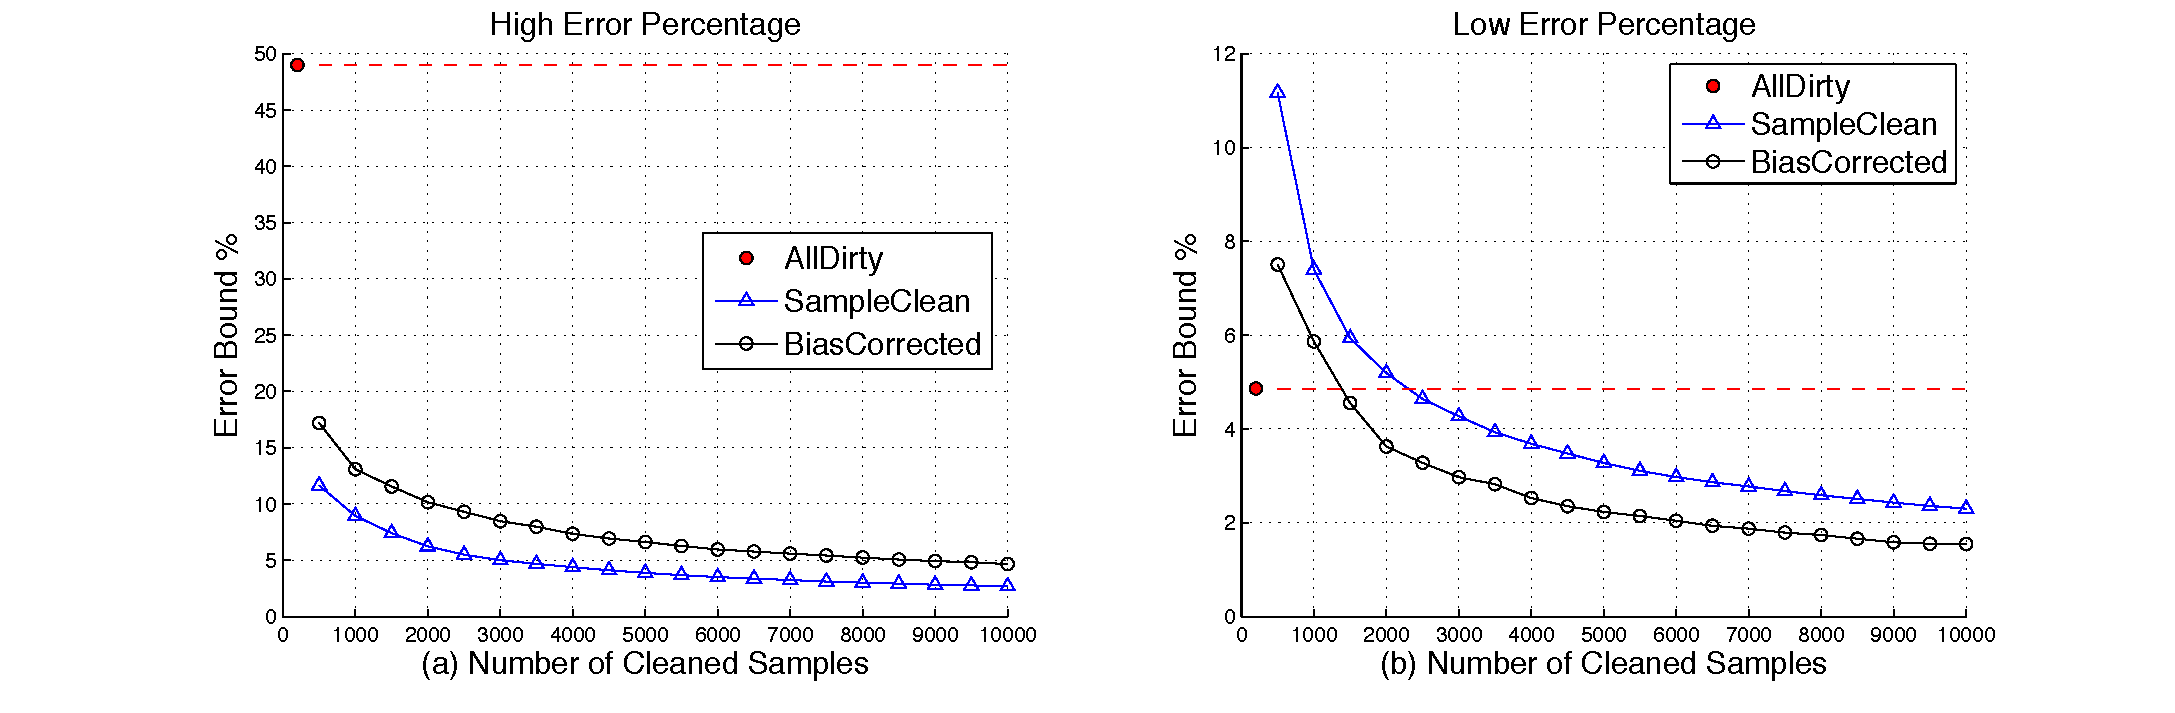
\includegraphics[width=.6\columnwidth]{figs/allerror-samplesize.pdf}
\caption{Comparison of the convergence of the methods on two TPC-H datasets of 6M tuples with simulated errors 50\% error and 5\% error. On the dataset with larger errors, the direct estimate gives a narrower confidence interval, and on the other the correction is more accurate. \label{fig:est2}}
\end{SCfigure}




\section{Proposals}
We first look at subproblem relevant to the pipeline optimization; how do we represent the relationships 
between tuples in these entity resolution tasks.
We call this intermediate data structure a proposal since metaphorically the data cleaning operations propose changes.
The execution engine then takes this proposal and formulates an actionable execution plan based on the proposal actually apply the changes.

The solution will be to break apart the ER operators in the previous section and represent their operations
as a graph.
In this section, we describe this procedure for a single given pipeline.
Then, we discuss how to merge different proposals.

\subsection{Building Proposals}
We re-define entity resolution in terms of what we call \emph{proposal operations}.
That is instead of making a change, the operation proposes a candidate change.
By exposing this intermediate state rather than immediate applying changes, we can relax some of the assumptions we made
in the previous section when formalizing entity resolution.

First, $\delta$ operations need not execute one-to-one merges.
We can propose a set of candidate merges e.g. row1 one is linked to row2 and row3.
Similarly, with $\kappa$ operations we can propose a set of possible transformations e.g. if my attribute is a comma separated string value, the relevant data is either in 1st or 2nd field.
We can defer enforcing correctness to when the proposal is actually executed.
One way to think about this approach is that we are building a probabilistic database on a deterministic database and lazily marginalizing the distributions at execution time [cite].

\begin{definition} Entity Resolution Proposals. 
Proposal operations are functional operations on a weighted graph $G=(V,E,W(e),M(v))$ with edge weights $W(e)$ and a multiplicity function $M(v)$ for each vertex. 
Records in the database are represented as vertices, and proposed corrections/merges are represented as edges.
\begin{itemize}
\item Correct $\kappa(G,a_{1})$ For every $v \in V$, let $v'$ be the corrected version of $v$. We add $v'$ to $V$ if it does not exist and we draw an edge between $v$ and $v'$ with weight $w$ where a larger $w$ indicates increased confidence. If it already exists, we increment the multiplicty counter for $v'$. If $v$ has multiple possible corrected versions, repeat for all.
\item Deduplication $\delta(G)$ For every $v \in V$, draw an edge starting at $v$ to represent merging two records with weight $w$ where a larger $w$ indicates increased confidence. If it has multiple possible merges, draw edges for all.
\end{itemize}
%Like before, we constrain that $\kappa$ and $\delta$ are consistent; that is given two records that are identical on the projection their operation is identical.
\end{definition}

The end of a given pipeline will be a graph $G$. 
This graph structure is a generalization of the graph structure discussed in entity resolution [cite]; i.e. the graph in an open world model.

\subsection{Proposal API}
\reminder{TODO}

\subsection{Benefits from this Data Structure}
We list out some of the benefits of this data structure and what we can do with proposals that was not previously possible in pipeline of ``off-the-shelf" entity resolution components. First, proposals give a natural way to represent uncertainty using weighted edges. They also subsume deterministic algorithms as we can represent a tree of merges with uniform weights. It is true that internally, many ER algorithms use a similar construction, however, by building a single, unfied data structure to represent both $\kappa$ and $\delta$ operations, we can propagate the data structure through a pipeline of reusable components. 

The second benefit is a representation of history. 
By representing the $\kappa$ operations in the data structure, we do not lose history when we apply an operation.
For example, an operation might be correct for 80\% of records and give incorrect results for the last 20\%, and the data structure gives us a natural way to interface with previously correct results.

The practical implications of this structure are interesting. 
For example, in ER pipelines, we often have to make many decisions up front such as what string tokenizer to use, how to threshold heuristics, or how dates should be formatted.
In this model, with the proposal structure, we argue why not try all of them.
Obviously there is a trade-off space between ER accuracy and performance, and we will discuss that more in the next section.

\subsection{Proposal Overhead}
The proposal framework introduces overhead as the graph $G$ is much larger in terms of both edges and vertices than typically considered in graph based ER tasks. 
This warrants new algorithms to process this larger graph.
If $p$ is the number of steps in the pipeline, and $k$ is the average number of candidates $O(p^2k^2+V^2)$.
\reminder{TODO}

\subsection{Algebra Over Proposals}
Given two different proposals $G_1$ and $G_2$, we can define a merge operations to make them a single proposal.
\reminder{TODO}


\section{Efficiency With Sampling}\label{dist-samp}
The model update received a sample with probabilities $p(\cdot)$.
For any distribution where  $p(\cdot) > 0$, we can preserve correctness.
\sys uses a sampling algorithm that selects the most valuable records to clean with higher probability. 

\subsection{Oracle Sampling Problem}
Recall that the convergence rate of an SGD algorithm is bounded by $\sigma^2$ which is the variance of the gradient.
Intuitively, the variance measures how accurately the gradient is estimated from a uniform sample.
Other sampling distributions, while preserving the sample expected value, may have a lower variance.
Thus, the oracle sampling problem is defined as a search over sampling distributions to find the minimum variance sampling distribution.

\begin{definition}[Oracle Sampling Problem]
Given a set of candidate dirty data $R_{dirty}$, $\forall r \in R_{dirty}$ find sampling probabilities $p(r)$ such that over all samples $S$ of size $k$ it minimizes:
\[
\mathbb{E}(\|g_S - g^*\|^2)
\]
\end{definition}
It can be shown that the optimal distribution over records in $R_{dirty}$ is probabilities proportional to:
\[
p_i \propto \|\nabla\phi(x^{(c)}_i,y^{(c)}_i,\theta^{(t)})\|
\]
We provide proofs and theoretical justification in appendix, but intuitively, records with higher gradients should be sampled with higher probability as they affect the update more significantly.
However, this cannot exclude records with lower gradients as that would induce a bias hurting convergence.
The problem is that this optimal distribution leads to a chicken-and-egg problem:
the optimal sampling distribution requires knowing $(x^{(c)}_i,y^{(c)}_i)$, however, cleaning is required to know those values.

\subsection{Dirty Gradient Solution}
Such an oracle does not exist, and one solution is to use the gradient w.r.t to the dirty data:
\[
p_i \propto \|\nabla\phi(x^{(d)}_i,y^{(d)}_i,\theta^{(t)})\|
\]
It turns out that this solution works reasonably well in practice on our experimental datasets and has been studied in Machine Learning as the Expected Gradient Length heuristic \cite{settles2010active}.
The contribution in this work is integrating this heuristic with statistically valid updates.
However, inutively, approximating the oracle as closely as possible can result in improved priortization.
The subsequent section describes two components, the detector and estimator, that can be used to achieve this.
Our experiments suggest up-to a 2x improvement in convergence when using these optional optimizations (Section \ref{comp}).
\section{Efficient Execution of Ensembled Pipelines}
\reminder{TODO}
\section{Streaming Progressive Correlation Clustering}
Given a graph $G = (V, E, W(e), M(v))$, we need to translate $G$ into actual changes to the tuples in the database.
In particular, we need to assign vertices to clusters -- each cluster represents an entity, and vertices in the cluster are duplicates of that entity.

We also want to provide low-latency intermediate results as the graph is updated in a streaming setting.

Currently, this is solved in SampleClean using connected components, which is prone to making significant errors in the presence of erroneous edges.

This problem has also been studied in the context of correlation clustering, a discrete optimization problem that attempts to find an assignment $\chi_{OPT}$ of vertices $v\in V$ to clusters satisfying
\[
\chi_{OPT} = \underset{\chi: V \rightarrow \mathbb{Z}}{\arg\min} \sum_{v \in V} \sum_{u \neq v} \mathbb{I}((u,v) \in E \oplus \chi(u) = \chi(v))
\]
where $\oplus$ is the exclusive-or operator.
That is, we wish to minimize the disagreements between the clustering $\chi$ and the graph $G$.

A simple randomized approximation algorithm is \emph{KwikCluster} [cite]. \reminder{Describe serial algorithm.}
\emph{KwikCluster} guarantees a 3 approximation, in expectation, to the correlation clustering problem for unweighted graphs.

However, this algorithm is serial and thus ill-suited for providing low-latency streaming results.
In this section, we explore parallel and streaming versions of KwikCluster.
Upon receiving a graph, the parallel KwikCluster implementation quickly returns a serializable clustering result;
as new vertices and edges are streamed in, the streaming algorithm updates the result in an eventually consistent fashion.

      \begin{algorithm}[h]
        \DontPrintSemicolon
        \caption{{\it KwikCluster}: serial peeling}
        \label{alg:seqgreedy}
        Init $\forall v\in V, \chi_{ser}(v) = \infty$\;
        Init $\forall v\in V, \gamma_{ser}(v) = $ UNASSIGNED\;
        \For {$i = 1$ to $n$}{
          Let $v$ be vertex such that $\pi(v) = i$.\;
          \If {$\gamma_{ser}(v) == $ UNASSIGNED}{
            $\gamma_{ser}(v) = $ CENTER\;
            $\chi_{ser}(v) = \pi(v)$\;
            \For {$u: (u,v) \in E^+$}{
              \If {$\gamma_{ser}(u) == $ UNASSIGNED}{
                $\gamma_{ser}(u) = $ SPOKE\;
                $\chi_{ser}(u) = \pi(v)$
              }
            }
          }
        }
      \end{algorithm}

\subsection{C4: Correlation Clustering using Concurrency Control}

We treat each set of KwikCluster operations on a vertex as an atomic transaction, and apply concurrency control mechanisms to ensure serializability.

C4 is guaranteed to be serializable.

      \begin{algorithm}[h]
        \DontPrintSemicolon
        \caption{{\it C4}: Parallel peeling}
        \label{alg:pargreedy}
        Init $\forall v\in V, \chi_{C4}(v) = \infty$\;
        Init $\forall v\in V, \gamma_{C4}(v) = $ UNASSIGNED\;
        \ParForAll{$p \in \{1, \ldots, P\}$}{
          \For {$i = p, p+P, \ldots, p + \lfloor n/P \rfloor P$}{
            \tcp{Transaction $T_v$}
            Let $v$ be vertex such that $\pi(v) = i$.\;
            \If {$\gamma_{C4}(v) == $ UNASSIGNED}{
              \tcp{Check concurrent neighbors}
              isCenter = {\scriptsize{\texttt{verifyIsCenter}}}($v$)\;
              \tcp{Create cluster}
              \lIf {isCenter}{
                {\scriptsize{\texttt{createCluster}}}($v$)
              }
            }
          }
        }
      \end{algorithm}

      \begin{algorithm}[h]
        \DontPrintSemicolon
        \caption{\texttt{verifyIsCenter($v$)}}
        \label{alg:verifyiscenter}
              \For {$u: (u,v) \in E^+$}{
                \If {$\pi(u) < \pi(v)$}{
                  \WaitUntil $\gamma_{C4}(u) \neq $ UNASSIGNED\;
                  \If {$\gamma_{C4}(u) == $ CENTER}{
                    return $false$
                  }
                }
              }
              return $true$
      \end{algorithm}
      \begin{algorithm}[h]
        \DontPrintSemicolon
        \caption{\texttt{createCluster($v$)}}
        \label{alg:createcluster}
        $\gamma_{C4}(v) = $ CENTER\;
        $\chi_{C4}(v) = \pi(v)$\;
        \For {$u: (u,v) \in E^+$}{
          \tcp{Atomic check \& set}
          \If {$\chi_{C4}(u) > \pi(v)$}{
            $\gamma_{C4}(u) = $ SPOKE;
            $\quad\chi_{C4}(u) = \pi(v)$
          }
        }
      \end{algorithm}


\subsection{EC3: Eventually Consistent Correlation Clustering}


\section{Results}
Use three datasets for which we have some ground truth. They are all small

Comparison: Pr* (Optimal single pipeline), RPr (All samples of EPS), RPr-50 (50\% of EPS samples), Pr- (worst pipeline), and baseline* (Jiannan's Crowder Clustering algorithm but using the best sequence of actions).

\subsection{Does Randomization Make Pipelining More Robust?}
Compare to best single pipeline, worst single pipeline, and current state of the art.
We should find that a randomized execution is much better than the worst and hopefully comparable to the best.
In some cases, it may be better than the best, but it should never be worse than the worst.

Dataset: MS Academic 
Operations: Filter and Deduplicate

Dataset: Yelp 
Operations: String Clean, City Format, Deduplicate

Dataset: Product 
Operations: identify sku if exists, string clean, Deduplicate

\begin{figure}[ht]
\centering
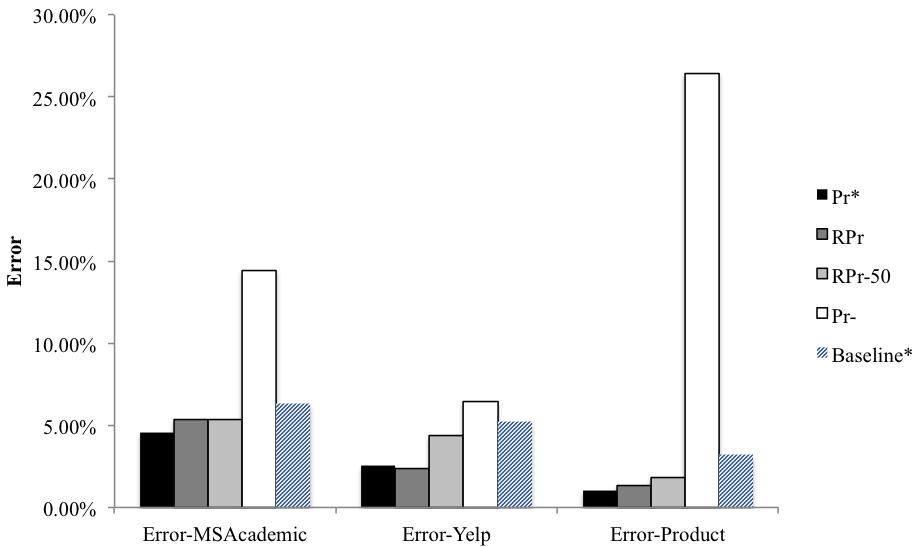
\includegraphics[scale=0.4]{fig1.png}
\caption{}
\label{exp:ms-academic-ranking}
\end{figure}

\subsection{How does this vary with random error in the operators?}
Should show that the more unreliable the data cleaning is the more that our approach benefits.

Introduce varying amount of random error (hashed so consistent between runs) into the ``city formatting" fix for the yelp dataset:

\begin{figure}[ht]
\centering
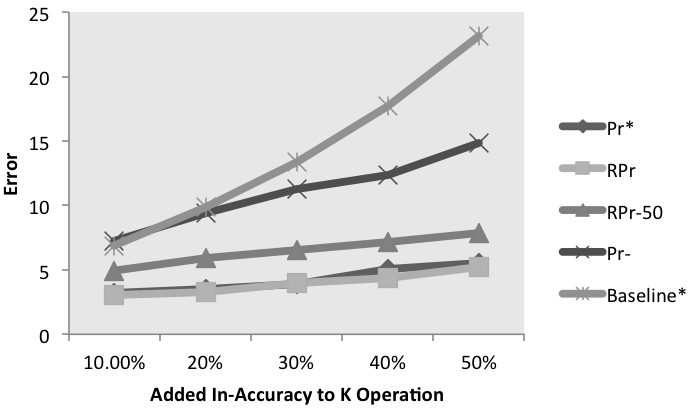
\includegraphics[scale=0.5]{fig2.png}
\caption{}
\label{exp:ms-academic-ranking}
\end{figure}

Introduce varying amount of random error (hashed so consistent between runs) into an extra dedup operation.

\begin{figure}[ht]
\centering
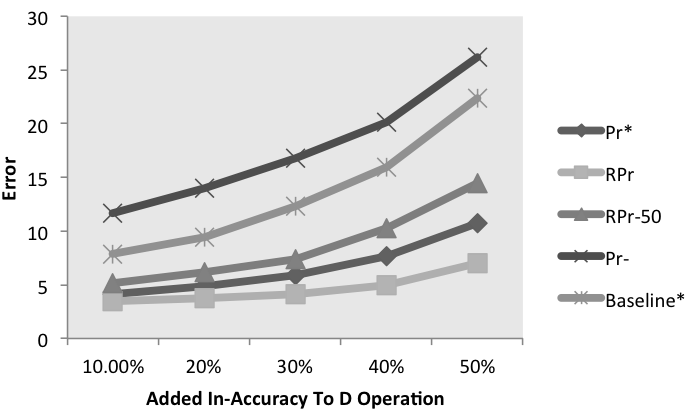
\includegraphics[scale=0.5]{fig3.png}
\caption{}
\label{exp:ms-academic-ranking}
\end{figure}

\subsection{Runtime-Accuracy Tradeoff}
Execute more samples and show how the accuracy improves.

\begin{figure}[ht]
\centering
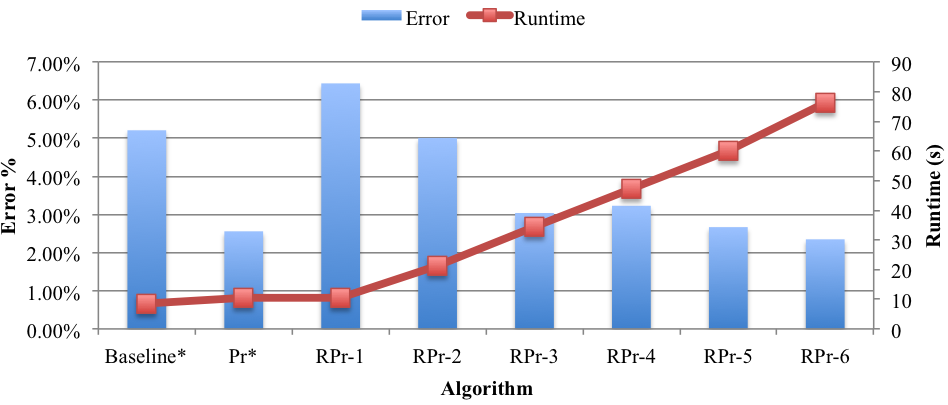
\includegraphics[scale=0.5]{fig4.png}
\caption{}
\label{exp:ms-academic-ranking}
\end{figure}


\subsection{Large-scale experiments}
Streaming correlation clustering. Show that at scale this technique can work and in a distributed environment.
In order to quantify the robustness of our methodology, we intend to run the algorithm on both synthetic and realworld datasets.
The synthetic dataset give us the ability to control the parameters while explore the state of possible responses.
However, a pitfall with such analysis is it's rather difficult to measure actual improvement over random fluctuations as well as the improvement may not be uniform across all tasks.
With experimentation on the real world datasets, we indent to first show the applicability of our method; and secondly determine whether results from our previous analysis extends to non-synthetic scenarios.



\vspace{-.5em}
\section{Conclusion and Future Work}\label{sec:con}
In this paper, we explore using sampling, integrated with data cleaning, to improve answer quality. We propose \saqpplus, a novel framework which only requires users to clean a sample of data, and utilizes the cleaned sample to obtain unbiased query results with confidence intervals.
We identify three types of data errors (i.e., value error, condition error and duplication error) that may affect query results, and develop \biascorrected and \sampleclean to estimate query results for the data with these errors.
Our analysis and experiments suggest that \saqpplus, which returns the better result between \biascorrected and \sampleclean, is robust to different magnitudes and rates of data errors, and consistently reports good estimate results.
%Moreover, \saqpplus can optimally satisfy user-specified cleaning-cost or result-quality constraints.
Our experiments on both real and synthetic data sets indicate that \saqpplus only needs to clean a small sample of the data to achieve accurate results, and furthermore the size of this sample is independent of the size of the dataset.
In particular, \sampleclean, which processes queries only on the cleaned sample, not only makes the query processing more scalable, but surprisingly may provide higher quality results than an aggregation of the entire dirty data (\alldirty).

To the best of our knowledge, this is the first work to marry data cleaning with sampling-based query processing.
%But, it is merely the tip of the iceberg.
There are many research directions for future exploration. 

\vspace{.25em}
{\noindent \bf Constrained Queries:} Now that we have quantified a tradeoff between cleaning costs and result quality, we can explore query results where users can specify a cost or quality constraint. For example, users may want to know that given a cleaning budget, what is the best result quality they can achieve? Or, given a quality constraint, how many samples they need clean to meet the constraint? 
In these constrained queries, we aim to answer with an optimal cost or most accurate result to meet the constraints.

\vspace{.25em}
{\noindent \bf Uncertain Cleaning Results:}  Our framework can return unbiased query results with respect to AllClean for a variety of different data cleaning approaches.
We are also interested in how we can incorporate uncertain or probabilistic cleaning processes into this framework.
For example, given a dirty record, could the data cleaning module specify a set of ranges for each attribute? 
We are interested in what guarantees, if any, we can achieve in such settings.

\vspace{.25em}
{\noindent \bf Complex SQL Queries:} Another important avenue of future work is to extend our framework to support more complex SQL queries such as join and nested SQL queries. There are some straightforward methods to implement these queries. For example, we can materialize the join result as a single table, and then apply our framework to the materialized table. But this could be very costly for large datasets, thus we need to explore more efficient implementations.
For a larger set of queries, it may not be possible to estimate their results with the CLT.
Thus, exploring empirical estimation approaches (such as bootstrapping) to our framework is another interesting future direction.

\vspace{.25em}
{\noindent \bf Sample Maintenance:} Finally, in real applications users may create multiple samples from the data.
Maintaining these samples for data updates is also very challenging and needs to be investigated.


\vspace{1.5em}

\fussy
{\noindent  \bf Acknowledgements.} {\small  The authors would like to thank Sameer Agarwal, Bill Zhao, and the SIGMOD reviewers for their insightful feedback. This research is supported in part by NSF CISE Expeditions Award CCF-1139158, LBNL Award 7076018, DARPA XData Award FA8750-12-2-0331, the European Research Council under the FP7, ERC MoDaS, agreement 291071, and by the Israel Ministry of Science, and gifts from Amazon Web Services, Google, SAP, The Thomas and Stacey Siebel Foundation, Apple, Inc., Cisco, Cloudera, EMC, Ericsson, Facebook, GameOnTalis, Guavus, Hortonworks, Huawei, Intel, Microsoft, NetApp, Pivotal, Samsung, Splunk, Virdata, VMware, WANdisco and Yahoo!.
}
\sloppy





\bibliographystyle{abbrv}
%\scriptsize
\fontsize{6.08pt}{6.4pt} \selectfont

\bibliography{er,crowdsourcing,stats,bigdata} 



\end{document}
